\section{Root Finding}
\label{Root Finding}

\begin{frame}{Converging on the "Right" Model}
Exhaustive iteration can be used for this analysis. However, we would need tens
of thousands of simulations per vernier scan beam displacement, set at a
granularity of the uncertainty of the parameters which we vary. \\~\\
With unlimited CPU priority on condor, this would not be a problem. However,
CPU time IS limited, and might require hundreds of CPU hours to use exhaustive
iteration.\\~\\
There is a better way - the simple binary search!
\end{frame}

\begin{frame}{Just in Case...}
\begin{figure}
\begin{center}
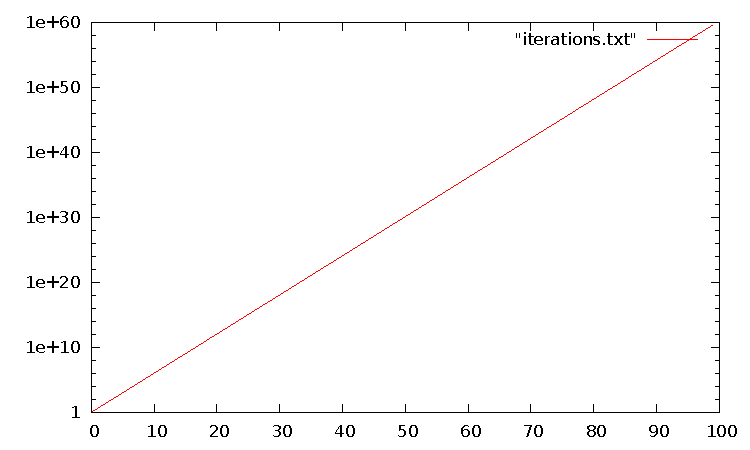
\includegraphics[width=0.7\linewidth]{../RootFinding/figs/iterations.pdf}
\end{center}
\caption{
	I expect to have four free parameters in this simulation. Shown is the number
	of simulation instances required to explore all parameters (vertical) vs the
	granularity of a single variable. Even with a meager granularity of 50,
	exhaustive iteration would require 4.9 CPU-years }
\label{fig:iterations}
\end{figure}
\end{frame}


\begin{frame}{Binary Search Introduction}
\textbf{Algorithm:}
\begin{itemize}
	\item Choose appropriate ranges for each parameter in the search 
	\item Step 1: Define a "step-size" whose initial value is 1/4 of the total
		variable range
	\item Step 2: Run simulation for all combinations of variables stepped once
		in positive and negative directions, relative to the central value of the
		step, in an increment of "step-size"
	\item Step 3: Choose combination of variables which minimizes the
		least-squared difference between simulated results and the data
	\item Step 4: Half the "step-size" for each variable
	\item Step 5: Return to step 2 with new "step-size"
\end{itemize}
We can stop the iteration arbitrarily, based on various constraints. For
example, we can stop iteration once the step size in the variable becomes
smaller than the variable's uncertainty. Or we can stop the iteration when we
reach a suitably small least-squares difference.
\end{frame}

\begin{frame}{ Starting With Maximum Overlap }
	\begin{itemize}
		\item From Figure~\ref{fig:359711_step_6_zvertex_compare}, we saw that
			convergence was very bad, perhaps indicating that bunches were not
			colliding centrally 
		\item However, we showed that the bunches do indeed cross at their central
			maximum.
		\item We show here the result of using the binary search to find the best
			set of parameters.
		\item Parameters varied: $\sigma_{x}$, $\beta^{*}$, $\theta_{XZ}$, and $N_{MC}$
	\end{itemize}
\end{frame}

\begin{frame}{Convergence of the Least-Squares Difference }
\begin{figure}
\begin{center}
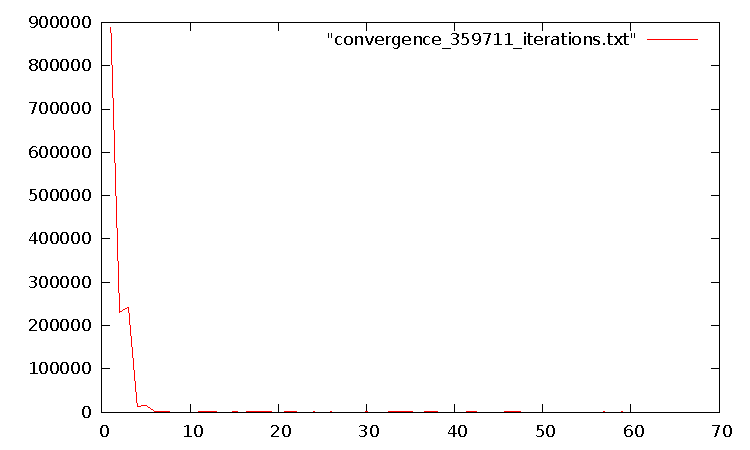
\includegraphics[width=0.8\linewidth]{../RootFinding/figs/convergence_359711_iterations.pdf}
\end{center}
\caption{We see the rapid convergence typical of a successful binary search.
Here, the criteria for convergence is one where the least-squares difference
between the simulation and data is less than 0.1. This can lead to many
iterations - in this case, the iteration was stopped manually once the
convergence value stopped changing. Axes are convergence parameter vs iterations}
\label{fig:convergence_359711_iterations}
\end{figure}
\end{frame}

\begin{frame}{Convergence of $\theta_{XZ}$ }
\begin{figure}
\begin{center}
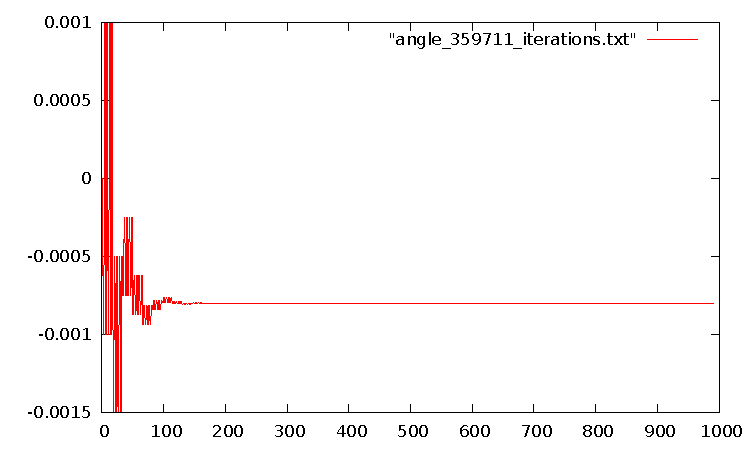
\includegraphics[width=0.8\linewidth]{../RootFinding/figs/angle_359711_convergence.pdf}
\end{center}
\caption{We can see the rapid fluctuations in $\theta_{XZ}$ as the code shifts
the value many times for each single iteration in various combinations. Axes are
parameter value vs number of simulations}
\label{fig:angle_359711_convergence}
\end{figure}
\end{frame}


\begin{frame}{Convergence of $\sigma_{x}$ }
\begin{figure}
\begin{center}
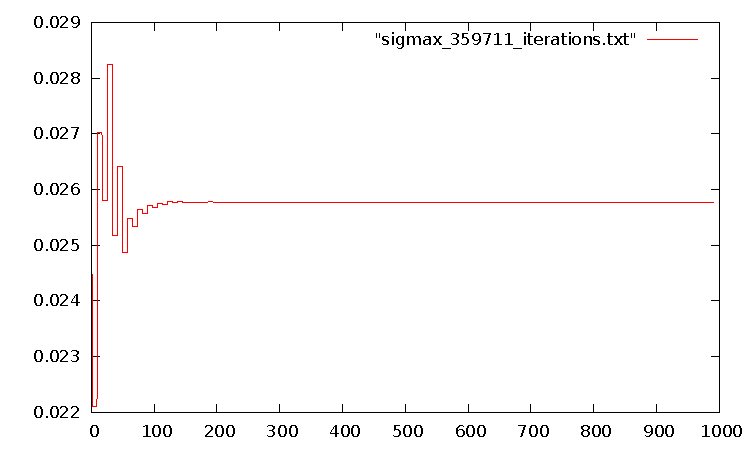
\includegraphics[width=0.8\linewidth]{../RootFinding/figs/sigmax_359711_convergence.pdf}
\end{center}
\caption{ 
Maximally overlapped beams will have more collisions per bunch crossing than
maximally displaced beams, which affects the overall beam-width fit. Until we
correct the rate data, we must treat $\sigma_{x}$ as a free parameter. Axes are
parameter value vs number of
simulations}
\label{fig:sigmax_359711_convergence}
\end{figure}
\end{frame}

\begin{frame}{Convergence of Collisions per Bunch Crossing}
\begin{figure}
\begin{center}
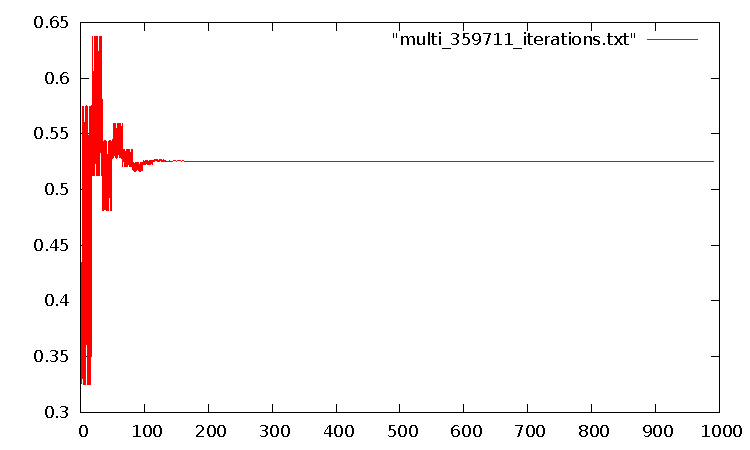
\includegraphics[width=0.8\linewidth]{../RootFinding/figs/multi_359711_convergence.pdf}
\end{center}
\caption{Normally, the collisions per bunch crossing is a separate correction
outside of the hourglass correction. But, here, we demonstrate that we do not
need this correction, if we have a reasonable starting value. In this case, I
use the Run 15 value (from 200 $GeV$ running) as a starting point. Axes are
parameter value vs number of simulations}
\label{fig:multi_359711_convergence}
\end{figure}
\end{frame}

\begin{frame}{ Convergence of $\beta^{*}$ }
\begin{figure}
\begin{center}
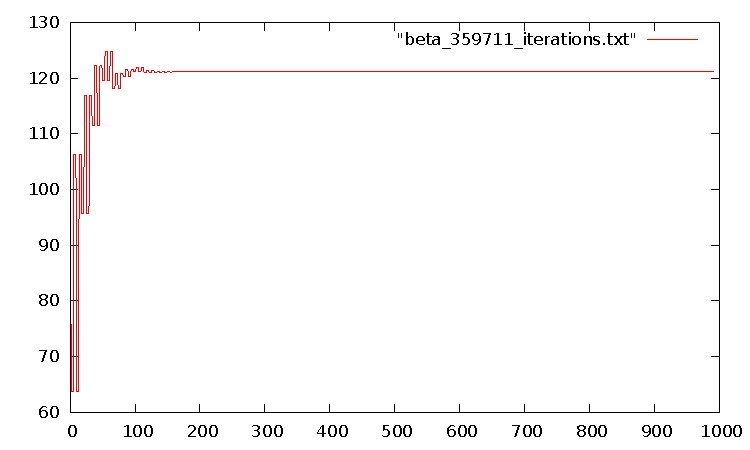
\includegraphics[width=0.8\linewidth]{../RootFinding/figs/beta_359711_convergence.pdf}
\end{center}
\caption{Finally, we have the value of $\beta^{*}$. Since we have discussed that
this value can vary as much as 50\% from run to run, I give it a broad
range. Axes are parameter value vs number of simulations}
\label{fig:beta_359711_convergence}
\end{figure}
\end{frame}

\begin{frame}{ Binary Search Results: Run 359711, Maximally Overlapped Beams (0 microns)}
\begin{figure}
\begin{center}
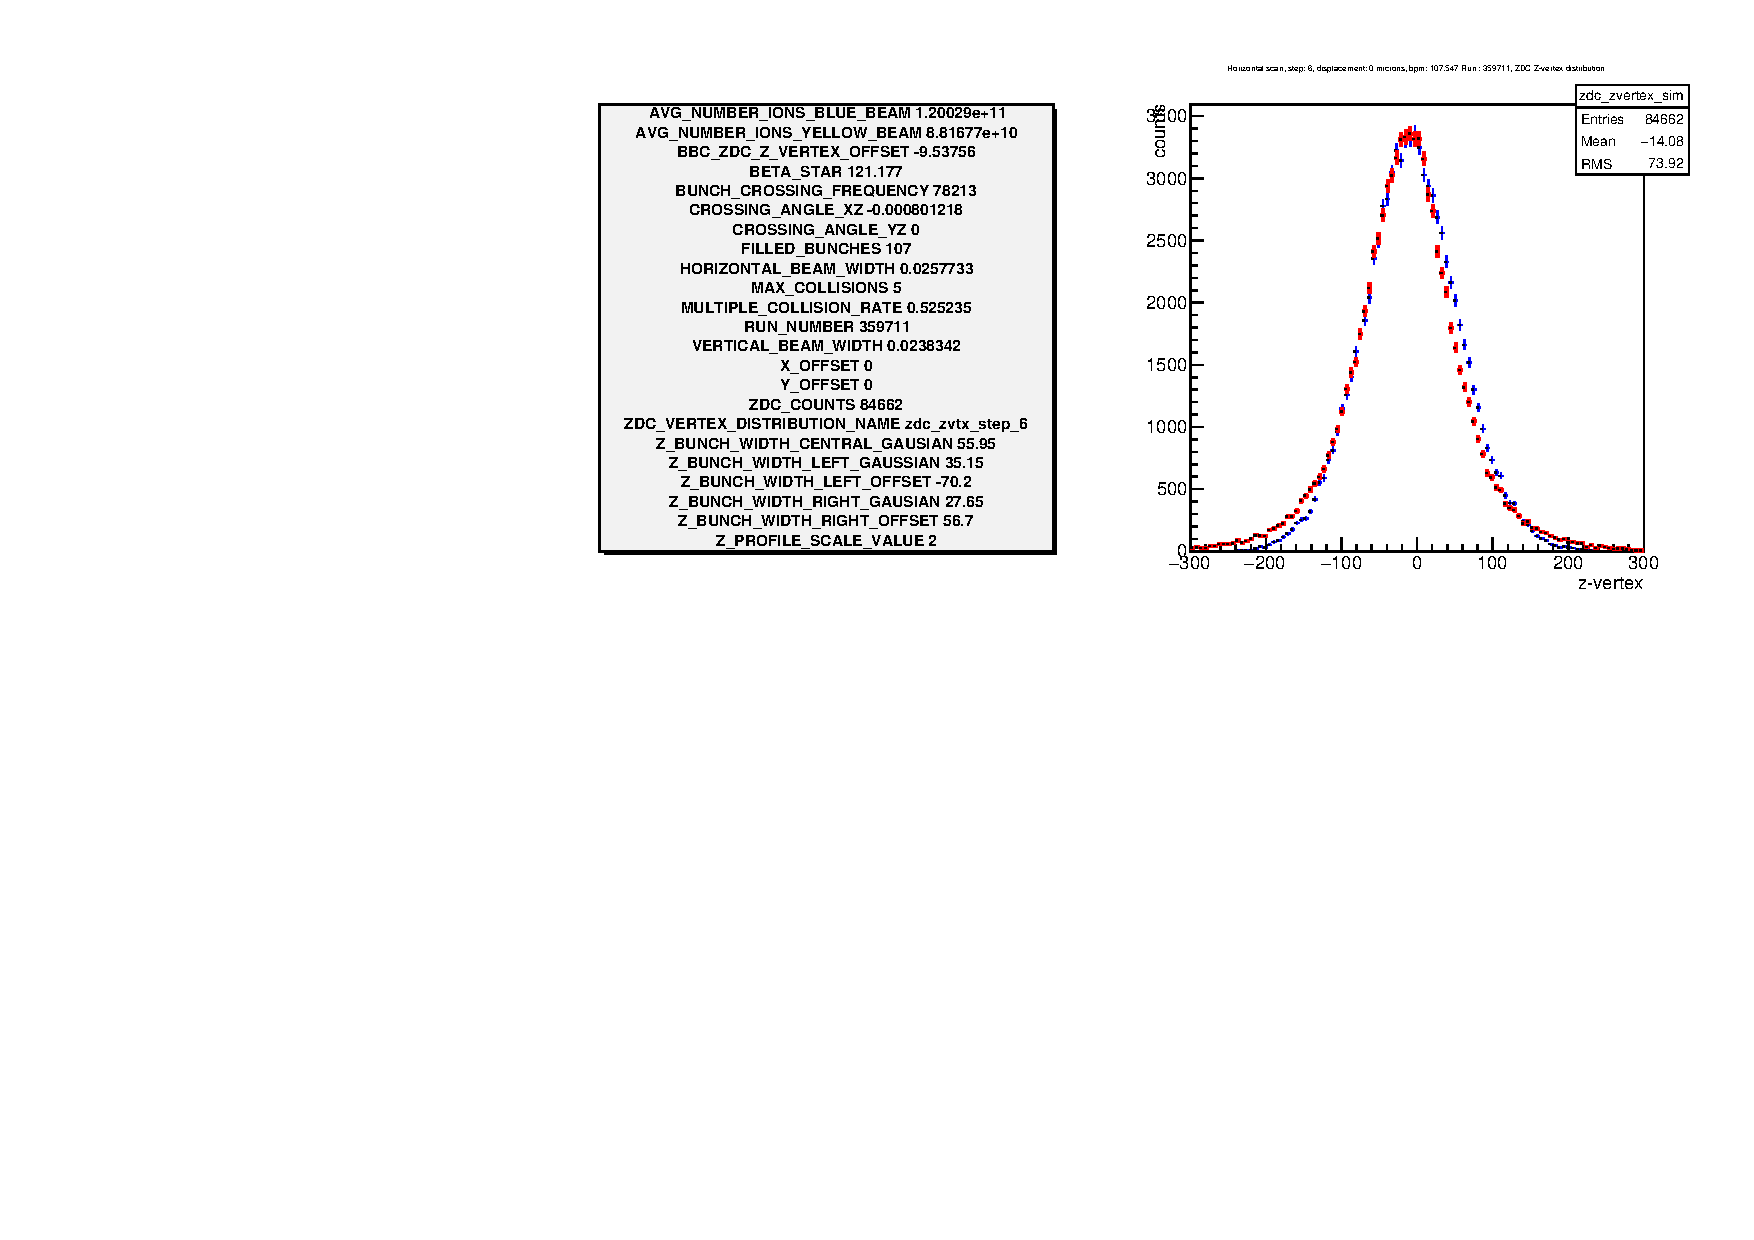
\includegraphics[width=\linewidth]{../RootFinding/figs/359711_max_overlap_binary_search.pdf}
\end{center}
\caption{Binary search vastly improves the convergence, but we can see it isn't
perfect. Are we happy with this, or does this warrant further investigation?}
\label{fig:359711_max_overlap_binary_search}
\end{figure}
\end{frame}

\begin{frame}{ Binary Search Results: Run 359711, Maximally Displaced Beams (-1000 microns) }
\begin{figure}
\begin{center}
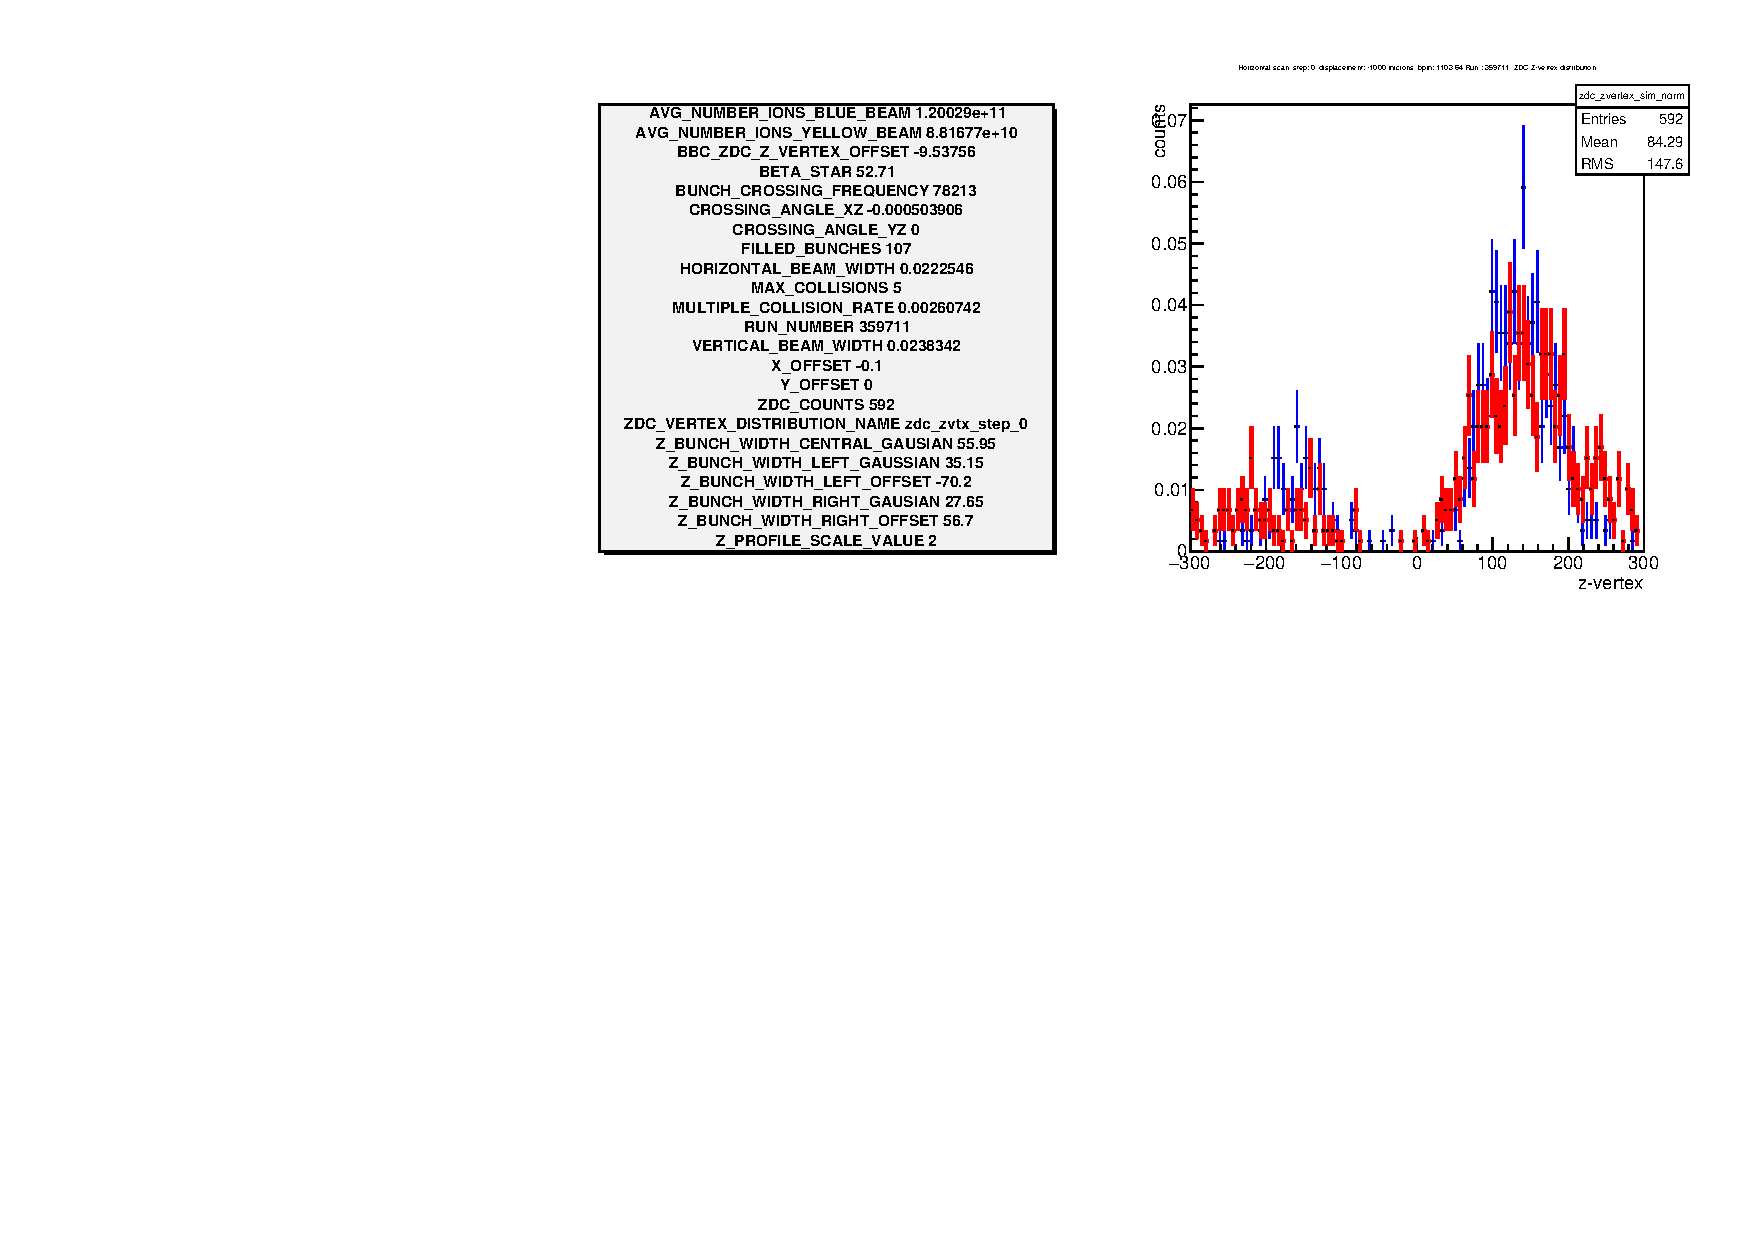
\includegraphics[width=\linewidth]{../RootFinding/figs/359711_min_overlap_binary_search.pdf}
\end{center}
\caption{Binary search vastly improves the convergence, but we can see it isn't
perfect. Are we happy with this, or does this warrant further investigation?}
\label{fig:359711_min_overlap_binary_search}
\end{figure}
\end{frame}

